

In order to solve real life tasks with high-velocity data, the stream processing systems can be used as a solution. The good example of such distributed model is FlameStream \cite{Kuralenok:2018}. FlameStream provides the following advantages:

\textbf{Determinism.} The result of computing is determined only by input data and remain the same between independent launches. This makes whole classifying process more predictable. In addition, the concept ensures an opportunity for tests that validate the whole pipeline.

\textbf{Low latency.} Unlike the other stream processing systems such as Apache Flink [?], Google's MillWheel [?], Spark Streaming[?] or Apache Storm, FlameStream produces results with lower latency using the same data processing.

These advantages allows us to create a classifier with better performance and due to the determinism and exactly-once delivery guarantee ensures a consistent results.

Similar to other stream processing systems, FlameStream is doing its calculations using a computational graph. The graph provides a scheme of data flow and can be presented like this:

\begin{figure}[htbp]
  \centering
  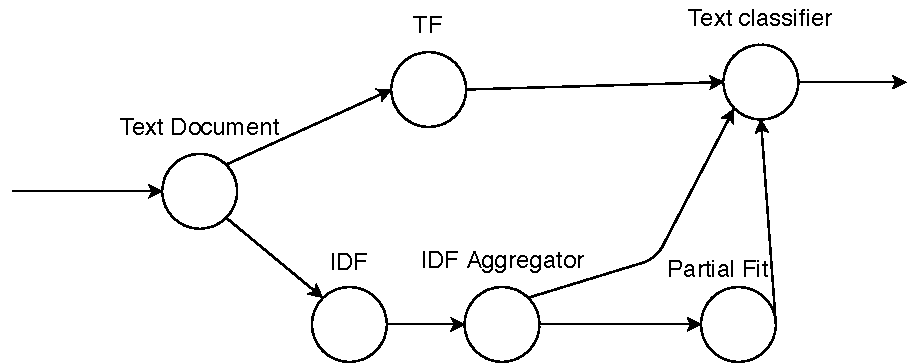
\includegraphics[scale=0.5]{pics/tf-idf-graph}
  \caption{The computational pipeline}
  \label {TF-IDF Graph}
\end{figure}

The Figure 1 illustrates our pipeline. An oriented edge indicates the flow of data. Every vertex in the graph represents a processing unit such as a single computer or a cluster. On the top of each vertex is a type of data, which the vertex is produce further. The initial text document splits into two computations: the first is calculates term frequencies and the second calculates inverse document frequencies. Results from IDF vertex aggregates and text classifier receives TF-IDF features of the document and produces result based on Logistic Regression model. The initial classifier weights provided by a pretrain process.

In addition, the Figure 1 provides a scheme for a partial fitting. Some of the text documents is labelled and such documents accumulate in the corresponding vertex. When the amount of new texts is enough for additional training, the existing classifier's weights are being updated as it is described below. After that, new weights is distributed among the system and process of classification continues. 

Further fitting process works according Multinomial Logistic Regression model, where cost function can be illustrates as follows(FIX THE FORMULA):

$$J(W) = -\frac{1}{m} \cdot \sum \limits_{i = 1}^{m} \sum \limits_{j = 1}^{k} \mathbbm{1}_{y^{(i)} == j} \cdot \log \frac{e^{W_{j}^Tx^{(i)}}}{\sum \limits_{l = 1}^{k}  e^{W_{l}^Tx^{(i)}}} + \lambda_1 ||W||_1 + \lambda_2 ||W - W_{prev}||_2 $$

The number of points in new dataset is denoted as $m$. The number of classes is $k$. New weights are designated as $W$ and previous weights are $W_{prev}$.

The gradient of the cost function can be put as(FIX TOO):

$$ \nabla_{W_j} J(W) = -\frac{1}{m} \cdot \sum \limits_{i = 1}^{m} [ x^{(i)} ( \mathbbm{1}_{y^{(i)} == j} - \frac{e^{W_{j}^Tx^{(i)}}}{\sum \limits_{l = 1}^{k}  e^{W_{l}^Tx^{(i)}}} ) ] $$

We calculate the gradient of each component and update the weights in one iteraton of the gradient descent. Maximum number of iterations of the descent is 100.